%% Benötigte Pakete
\RequirePackage{fix-cm} 

%% Dokumentendefinition für scrarticl. Optionen sind:
% a4paper, 	-?: Papierformat einstellung für Dokument
% 11pt, 	-?: 
\documentclass[ngerman, a4paper, 11pt]{scrartcl}

%% Konfiguration
% Hier werden alle Pakete importiert
%% Options
% Hier kommen alle Pakete hin

%% Deutesche Anpassungen
%
\usepackage[ngerman]{babel} 
\usepackage[utf8]{inputenc}
\usepackage[T1]{fontenc}    

%% Schrift Anpassungen
% Latin Modern Schriftart
\usepackage{lmodern}	%Latin Modern Schriftart
\renewcommand{\sfdefault}{\rmdefault}
\setkomafont{sectioning}{\rmfamily \bfseries} %Schriftart ändern
\setkomafont{descriptionlabel}{\rmfamily \bfseries}

%% Design Anpassungen
% Header Style für KOMA Script
\usepackage{scrpage2}
% Design Anpassungen
\usepackage{geometry}
% Optischer Randausgleich
\usepackage{microtype}	

%% Floats Optimierungen
% Behaltet floats im definierten bereich
\usepackage[section]{placeins}
\usepackage{float}


%% Ausrichtung
%
%\usepackage{minipage}
\usepackage{multicol}
% Für einzelne Seiten Querformat
\usepackage{lscape} 
\usepackage{placeins}

%% Bilder
%Zum Laden von Grafiken
\usepackage{graphicx}
\usepackage[justification=centerlast]{caption}
%Teilabbildungen in einer Abbildung
%\usepackage{subfigure}
%Teilabbildungen in einer Abbildung
%Besser als subfigure oder subfig
\usepackage{subcaption}



%% Listen
%
\usepackage{mdwlist}
\usepackage{paralist}
\usepackage{enumitem}
\renewcommand\labelitemi{--}

%% Tabellen
%
\usepackage{array}
\usepackage{tabularx}
\usepackage{booktabs}
% Für Tabellen, die eine Seite überschreiten
\usepackage{longtable} 
\usepackage{multirow}
\usepackage{makecell, boldline}
% Mit diesem Kommando kann in einer Tabelle die Zeile umgebrochen werden
% ... & \specialcell{aaa\\bbb} & \specialcell{aaa\\bbb} \\
\newcommand{\specialcell}[2][c]{%
	\begin{tabular}[#1]{@{}l@{}}#2\end{tabular}}

%% Mathe
%
\usepackage{amsmath} 
\usepackage{amsfonts}
\usepackage{amsthm}
%SI Einheiten usw.
%\usepackage[binary-units]{siunitx}

%% Code
\usepackage{listings}
%%
%\lstdefinestyle{tt}{basicstyle=\small\ttfamily,keywordstyle=\bfseries,language=[LaTeX]{TeX}}
%\lstdefinestyle{rm}{basicstyle=\ttfamily,keywordstyle=\slshape,language=[LaTeX]{TeX}}
%\begin{lstlisting}[style=tt]
%	\documentclass{foo}
%\end{lstlisting}

%% URL
%      
\usepackage{url}
\usepackage{breakurl}
\usepackage{color}
\usepackage[dvipsnames]{xcolor}

\usepackage{tikz}


% Farben
%
\usepackage{xcolor}

%% PDF
%
\usepackage{pdfpages}

%% Autonum Funktion
%
\usepackage{ifthen}       


%% Querverweise
\usepackage{appendix}
\usepackage{varioref}
\usepackage[
colorlinks,        % Links ohne Umrandungen in zu wählender Farbe
linkcolor=black,   % Farbe interner Verweise
filecolor=black,   % Farbe externer Verweise
citecolor=black,    % Farbe von Zitaten
urlcolor=black
]{hyperref}
\usepackage{cleveref}


%% Code
%% dieses Command stellt den Zäler \rowno bereit
% Mit \rowno[1] wird der Zäler wauf eins gesetzt
\makeatletter
\providecommand{\rowno}[1][__empty__]{%
	\ifthenelse{\isundefined{\c@rowno}}{%
		\newcounter{rowno}}{}%
	\ifthenelse{\equal{#1}{__empty__}}{%
		\stepcounter{rowno}%
	}{%
		\setcounter{rowno}{#1}%
	}%
	\therowno%
}
\makeatother
% Umbenennen der Referenz
\renewcommand{\lstlistingname}{Code-Snipped}% Listing -> Algorithm
\renewcommand{\lstlistlistingname}{Verzeichniss der \lstlistingname e}%
\crefname{listing}{\lstlistingname}{\lstlistingname e}  
\Crefname{listing}{\lstlistingname}{\lstlistingname e}


%% In diesem File werden alle Konfigurationen wie bspw. eine Programierumgebung konfiguriert
\definecolor{codegreen}{rgb}{0,0.6,0}
\definecolor{codegray}{rgb}{0.5,0.5,0.5}
\definecolor{codepurple}{rgb}{0.58,0,0.82}
\definecolor{backcolour}{rgb}{0.95,0.95,0.95}

\definecolor{lstRed}{rgb}{0.88,0.11,0.19} 
\definecolor{lstBlue}{rgb}{0,0,0.39}
\definecolor{lstGreen}{rgb}{0,0.55,0.27}
\definecolor{lstCyan}{rgb}{0.0,0.6,0.6}
\definecolor{lstWhite}{rgb}{0.99,0.99,0.99}
\definecolor{lstBlack}{rgb}{0.0,0.0,0.0}
\definecolor{lstGrey}{rgb}{0.39,.39,0.39}

\definecolor{CommentGreen}{rgb}{0.1,0.35,0.1}
\definecolor{Background}{rgb}{0.97,0.97,0.97}
\definecolor{lrow}{rgb}{0.914,0.918,0.922}
\definecolor{drow}{rgb}{0.725,0.745,0.769}

\lstloadlanguages{C,C++,csh,Java,SQL,Python,bash}

%%

\lstset{
	language=csh,
	basicstyle=\footnotesize\sffamily,
	numbers=left,
	numberstyle=\tiny,
	numbersep=5pt,
	tabsize=2,
	extendedchars=true,
	breaklines=true,
	frame=b,
	stringstyle=\color{lstBlack}\sffamily,
	showspaces=false,
	showtabs=false,
	xleftmargin=17pt,
	framexleftmargin=17pt,
	framexrightmargin=5pt,
	framexbottommargin=4pt,
	commentstyle=\color{lstGrey},
	morecomment=[l]{//}, %use comment-line-style!
	morecomment=[l]{///}, %use comment-line-style!
	morecomment=[s]{/*}{*/}, %for multiline comments
	showstringspaces=false,
	morekeywords={ abstract, event, new, struct,
		as, explicit, null, switch,
		base, extern, object, this,
		bool, false, operator, throw,
		break, finally, out, true,
		byte, fixed, override, try,
		case, float, params, typeof,
		catch, for, private, uint,
		char, foreach, protected, ulong,
		checked, goto, public, unchecked,
		class, if, readonly, unsafe,
		const, implicit, ref, ushort,
		continue, in, return, using,
		decimal, int, sbyte, virtual,
		default, interface, sealed, volatile,
		delegate, internal, short, void,
		do, is, sizeof, while,
		double, lock, stackalloc,
		else, long, static,
		enum, namespace, string},
	keywordstyle=\color{lstBlue},
	identifierstyle=\color{lstBlack},
	backgroundcolor=\color{lstWhite},
}

\lstset{
	language=C++,
	upquote=true, frame=single,
	basicstyle=\small\ttfamily,
	backgroundcolor=\color{Background},
	keywordstyle=[1]\color{blue}\bfseries,
	keywordstyle=[2]\color{purple},
	keywordstyle=[3]\color{black}\bfseries,
	identifierstyle=,
	commentstyle=\usefont{T1}{pcr}{m}{sl}\color{CommentGreen}\small,
	stringstyle=\color{purple},
	showstringspaces=false, tabsize=5,
	morekeywords={properties,methods,classdef},
	morekeywords=[2]{handle},
	morecomment=[l][\color{blue}]{...},
	numbers=none, firstnumber=1,
	numberstyle=\tiny\color{blue},
	stepnumber=1, xleftmargin=10pt, xrightmargin=10pt
}

\lstset{
	language= Python,
	backgroundcolor=\color{backcolour},   
	commentstyle=\color{codegreen},
	keywordstyle=\color{magenta},
	numberstyle=\tiny\color{codegray},
	stringstyle=\color{codepurple},
	basicstyle=\ttfamily\footnotesize,
	breakatwhitespace=false,         
	breaklines=true,                 
	captionpos=b,                    
	keepspaces=true,                 
	numbers=left,                    
	numbersep=5pt,                  
	showspaces=false,                
	showstringspaces=false,
	showtabs=false,                  
	tabsize=4
}


\lstset{literate=% Allow for German characters in lstlistings.
	{Ö}{{\"O}}1
	{Ä}{{\"A}}1
	{Ü}{{\"U}}1
	{ß}{{\ss}}2
	{ü}{{\"u}}1
	{ä}{{\"a}}1
	{ö}{{\"o}}1
}


%tikz
\usetikzlibrary{arrows.meta,positioning}

\bibliography{./bib/literaturBibLatex.bib}

\usepackage{bbding}



\begin{document}
	\titlehead{30526-01 – Introduction to Internet and Security 
	\
	\hfill  Projekt LoRa}
\title{
\includegraphics[width=6cm]{./thm/picLogo.eps}
	\\ \vspace{1em}
	Projekt-Dokumentation}
\author{Luc Heitz \flqq luc.heitz@unibas.ch\frqq \\
	Manuel  Schmidt \flqq manuel.schmidt@stud.unibas.ch\frqq \\
	Raphael Waltenspül \flqq raphael.waltenspuel@stud.unibas.ch
}

\date{\today}
\publishers{
	Universität Basel}
\maketitle

%\tableofcontents
	


\section{Einleitung}


\subsection{Vision}
Alternatives Netz, zum übertragen von Nachrichten, unabhängig von Internetprovider

\subsection{Ziel}
\begin{itemize}
\item LoRa Hardware, als Sender, Empfänger und Relais (Repeater)
\item Versenden von kleinen Textnachrichten
\item Peer to Peer mit Gossip-protokoll
\end{itemize}



\section{Verwendete Hardware}

\subsection{Hardwareaufbau}
Für den Hardwareaufbau wurden folgende Komponenten gewählt.

\begin{itemize}
	\item Raspberry Pi 3 Modell B 
	\item Dragino Lora/GPS Hat (Chip SX1276)
	\item 1 Raspberry mit Touchdisplay als Mobiler Empfänger
\end{itemize}


\textbf{Zusätzlich wurden Benötigt:}

\begin{itemize}
	\item Stromquelle für Aussen Tests (Powerbanks)
\end{itemize}

\Cref{fig:raspis} Zeigt den Aufbau mit und ohne Display


 \begin{figure}[H]
	\centering
	\begin{subfigure}[b]{.53\textwidth}
		\centering
		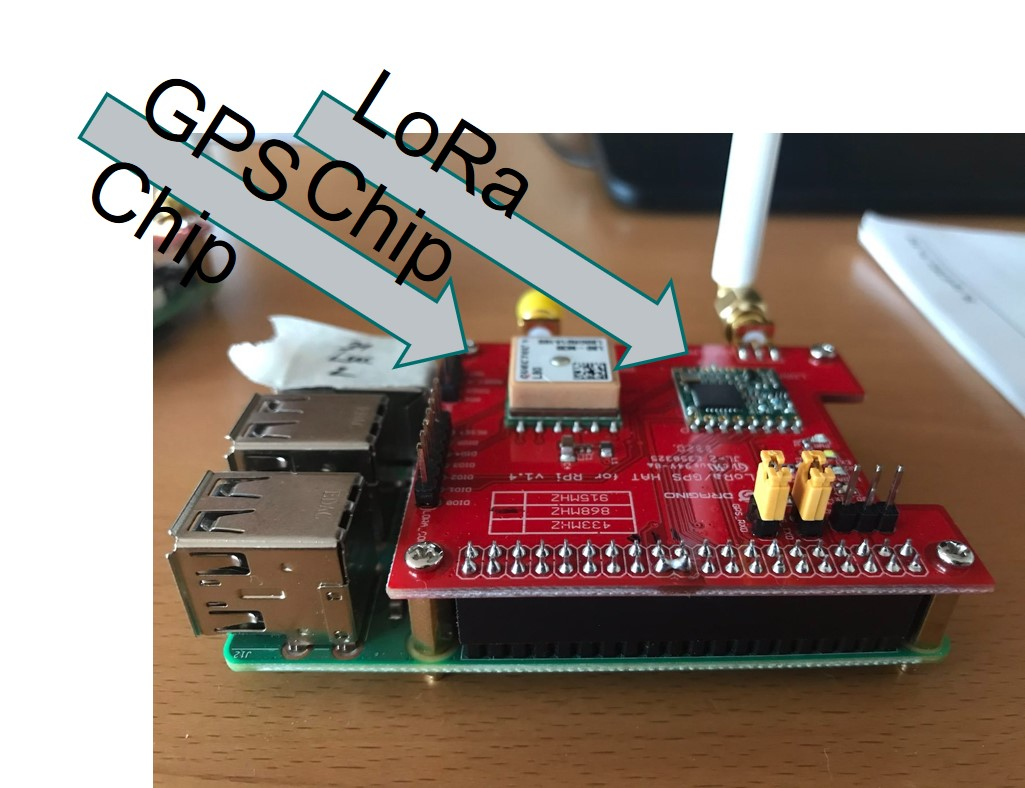
\includegraphics[width=\textwidth]{./pic/raspi1a}
		\caption{Raspi LoRa hat}
	\end{subfigure}
	\hfill
	\begin{subfigure}[b]{.45\textwidth}
		\centering
		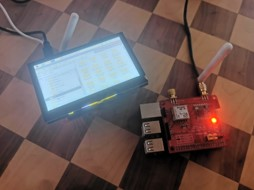
\includegraphics[width=\textwidth]{./pic/raspi2a}
		\caption{Version mit LCD display}
	\end{subfigure}
	
	\caption{Aufbau der Raspberry Pi LoRa Stationen}
	\label{fig:raspis}
\end{figure}

Die Kommunikation mit dem Chip SX1276 findet über einen SPI Bus statt. Das detailierte Schalt-Schema ist im \cref{app:schma} angefügt.
Weiter ist unter \href{https://wiki.dragino.com/index.php?title=Lora/GPS_HAT}{https://wiki.dragino.com/ index.php?title=Lora/GPS\_HAT} eine Dokumentation des Lora Hats als Wiki zu finden.




\subsection{Inbetriebnahme}
Erstes Ziel war das Raspberry Pi und Lora hat in Betrieb zu nehmen und über LoRa P2P Nachrichten an ein anderes Modul zu senden. 
Die Inbetriebnahme des Raspberry Pi zusammen mit dem LoRa hat gestaltete sich jedoch schwieriger als geplant. 

Es traten folgende Hauptprobleme auf:

\begin{description}
	\item[Fehler 1:] Keine Antwort auf dem SPI bus, das Signal wurde nicht durch den Chip SX1276 verarbeitet.
	\item[Ursache 1:] Der Chip Enable des LoRa SPI war auf einem anderen pin als der CE des Raspberry Pi's
	\item[Lösung 1:] Es wurde eine Lötbrücke zwischen pin 22 und 24 gesetzt.
\end{description}

Nun konnte eine Nachricht zwischen zwei Modulen gesendet werden.

\begin{description}
	\item[Fehler 2:] Nach kurzer Zeit stürzte der SPI bus ab und mit Senden und empfangen war vorbei.
	\item[Ursache 2:] Auf dem bus waren störungen durch den nich angeschlossen Pin.
	\item[Lösung 2:] Einerseits wurde ein Hearbeat resp. Watchdog implementiert, welcher das Board bei einem Spi Fehler neu started, andereseits wurden die Pins hardwareseitig entfernt um die Störungen auf dem Bus zu reduzieren.
\end{description}

Danach konnten über einen P2P Chat Nachrichten zwischen den Modulen versendet werden.

\subsection{Treiber / Link Layer}
Um die Hardware in das Gesamtsystem einzubinden, wurde das Lora Link Layer entwickelt.
Das Lora Link Layer implementiert den SX1276 Treiber.
Es bietet als Schnittstelle zwei Queues an, eine Rx-Queue und eine Tx-Queue.

Solange in der Tx-Queue kein Paket zum versenden ansteht, horcht das Link Layer und füllt alle über LoRa empfangenen Pakete in die Rx-Queue.
Will man etwas versenden, füllt man das Paket in die Tx-Queue. Das Link Layer schaltet den Modus automatisch um bis alle Pakte in der Tx-Queue versendet wurden.



\appendix
\section{Appendix}
\subsection{Schalt-Schema LoRa Hat}\label{app:schma}
\begin{figure}[H]
	\centering
	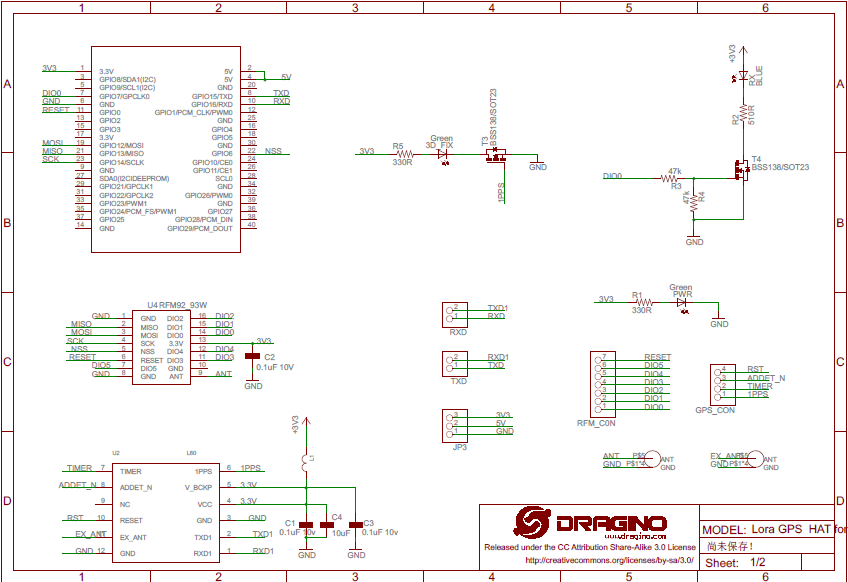
\includegraphics[width=0.99\linewidth]{./pic/GPS_HAT}
	\caption{Schema LoRa Hat}
	\label{fig:schema}
\end{figure}



\end{document}